\section{Tutorials}

\subsection{\LaTeX}

\begin{frame}
    \frametitle{Programmings in this class}
    \begin{itemize}
        \item \LaTeXs: 
            \begin{itemize}
                \item \texttt{moderncv}
                \item \texttt{beamer}
                \item \texttt{report}
                \item \href{http://www.texample.net}{\texttt{pgf/TikZ}}
            \end{itemize}
        \item Git
            \begin{itemize}
                \item \href{http://git-scm.com/doc}{\texttt{git gui}}
            \end{itemize}
        \item R:
            \begin{itemize}
                \item \texttt{lm}
                \item \href{https://catalyst.library.jhu.edu/catalog/bib_3642743}{\texttt{ggplot2}}
                \item \href{http://www.texample.net/tikz/examples/tikzdevice-demo/}{\texttt{tikzDevice}}
                \item \href{http://www.public.iastate.edu/~dicook/VIGRE/R-packages-slides.pdf}{\texttt{R CMD build}}
            \end{itemize}
    \end{itemize}
\end{frame}


\begin{frame}[fragile]
    \frametitle{Where to get some help for \LaTeXs}
    \begin{center}
    \href{http://en.wikibooks.org/wiki/LaTeX/}{http://en.wikibooks.org/wiki/LaTeX/}
    \end{center}
\end{frame}

\begin{frame}[fragile]
    \frametitle{Tutorial: \LaTeXs}
    \LaTeXs is a computer language for writing a scholarly paper:
    \begin{table}
        \centering
        \caption{HTML vs \LaTeXs}
        \begin{tabular}{c|p{3cm}|p{3cm}}
            \quad   &   HTML    & \LaTeXs \\ 
            \hline
            Code    & 
            \begin{lstlisting}
<html> 
 . . .
</html>
            \end{lstlisting} &  
            \begin{lstlisting}
\begin{document}
 . . .
\end{document}
            \end{lstlisting}\\
            \hline
            Compiler & Firefox and etc. & pdflatex and etc. \\
            \hline
            Output  & Web-page & PDF file
        \end{tabular}
        \label{tab:htmlvslatex}
    \end{table}
\end{frame}

\begin{frame}
    \frametitle{Tutorial: \LaTeXs}
    TeXworks is:
    \begin{itemize}
        \item an editing tool that is separate from \LaTeX,
        \item available in Linux, OSX and Windows,
        \item avaiable in: 
    \end{itemize}
    \vskip0.3in
    \begin{center}
    \href{http://code.google.com/p/texworks/}
    {http://code.google.com/p/texworks/}
    \end{center}
\end{frame}


\begin{frame}[fragile]
    \frametitle{Tutorial: \LaTeXs}
    \begin{itemize}
        \item Demo on preparing a resume using \LaTeXs \texttt{moderncv} package:
            \begin{itemize}
                \item Install \LaTeXs (MikTeX in Windows and MacTeX in OSX),
                \item Download \texttt{moderncv} package files from the course folder,
                \item Change file names to reflect you,
                \item Edit the TeX file,
                \item Compile using your favorite \LaTeXs editor,
                \item Look at the resulting PDF file.
            \end{itemize}
    \end{itemize}
\end{frame}

\begin{frame}[fragile]
    \frametitle{Tutorial: \LaTeX}
    Typing mathematics in \LaTeX:
    \begin{lstlisting}
Hello $\int_0^1 \sin(x) dx$ World
\vskip0.5in
Hello $$\int_0^1 \sin(x) dx$$ World
    \end{lstlisting}
    \vskip0.1in
Hello $\int_0^1 \sin(x) dx$ World
\vskip0.5in
Hello $$\int_0^1 \sin(x) dx$$ World
\end{frame}

\begin{frame}[fragile]
    \frametitle{Cautions: \LaTeXs}
    There are numerous quirky \LaTeXs rules:
    \begin{itemize}
        \item opening quotation is not the same as the closing quotation,
        \item period yields \emph{two} blank spaces, 
        \item for \%, need to type \verb+\%+,
        \item for \textbackslash, need to type \verb+\textbackslash+,
        \item for /, need to type /,
        \item for \{, need to type \verb+\{+,
        \item for \$, need to type \verb+\$+,
        \item \verb+~+ yields a single blank space,
        \item and etc.
    \end{itemize}
\end{frame}

\begin{frame}[fragile]
    \frametitle{Tutorial: \LaTeXs}
    How to make slides with notes:
    \begin{lstlisting}
\usepackage{handoutWithNotes}
\pgfpagesuselayout{4 on 1 with notes}[a4paper,border shrink=5mm]
    \end{lstlisting}
    This will 
    \begin{itemize}
        \item put four scaled-back slides in one page with ruled-note space on the right
        \item make the ``hyper links'' invalid
    \end{itemize}
    \vspace{1in}
\end{frame}


\subsection{Git}

\begin{frame}
    \frametitle{The place to get some Git helps}
    \begin{center}
        \href{http://git-scm.com/doc/}{http://git-scm.com/doc/}
    \end{center}
\end{frame}



\begin{frame}[fragile]
    \frametitle{Tutorial: Git}

\begin{lstlisting}
sudo apt-get install git
\end{lstlisting}

\begin{figure}[b]
    \caption{An alternative: \texttt{git gui}}
    \begin{center}
        
\includegraphics[height=0.6\textheight]{gitguiinstall.png}
    \end{center}
    \label{fig:gitgui}
\end{figure}
    
\end{frame}

\begin{frame}[fragile]
    \frametitle{Tutorial: Git}

\vspace{8pt}
\begin{lstlisting}
cd ~/
git clone http://cis.jhu.edu/~nhlee/550400.git
\end{lstlisting}

\begin{figure}[b]
    \caption{An alternative: \texttt{git gui}}
    \begin{center}
        
\includegraphics[height=0.5\textheight]{gitgui.png}
    \end{center}
    \label{fig:gitgui2}
\end{figure}
    
\end{frame}

\begin{frame}[fragile]
    \frametitle{Tutorial: Git}
\begin{lstlisting}
cd ~/550400
git reset --hard HEAD
git pull origin master
\end{lstlisting}
\begin{figure}[b]
    \centering
    \caption{An alternative: \texttt{git gui}}
        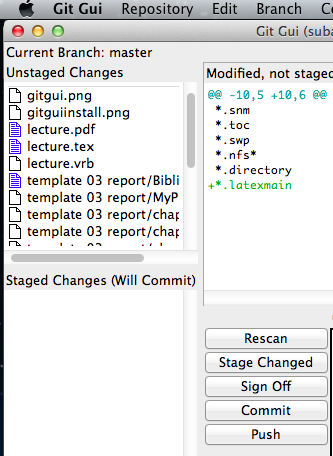
\includegraphics[height=0.6\textheight]{gitguiusing.png}
    \label{fig:gitgui4}
\end{figure}
\end{frame}



\begin{frame}[fragile]
    \frametitle{Tutorial: Git}
    After years of using git, you might find this funny: 
    \begin{columns}
        \begin{column}{0.5\textwidth}
            \begin{figure}
                \begin{center}
                    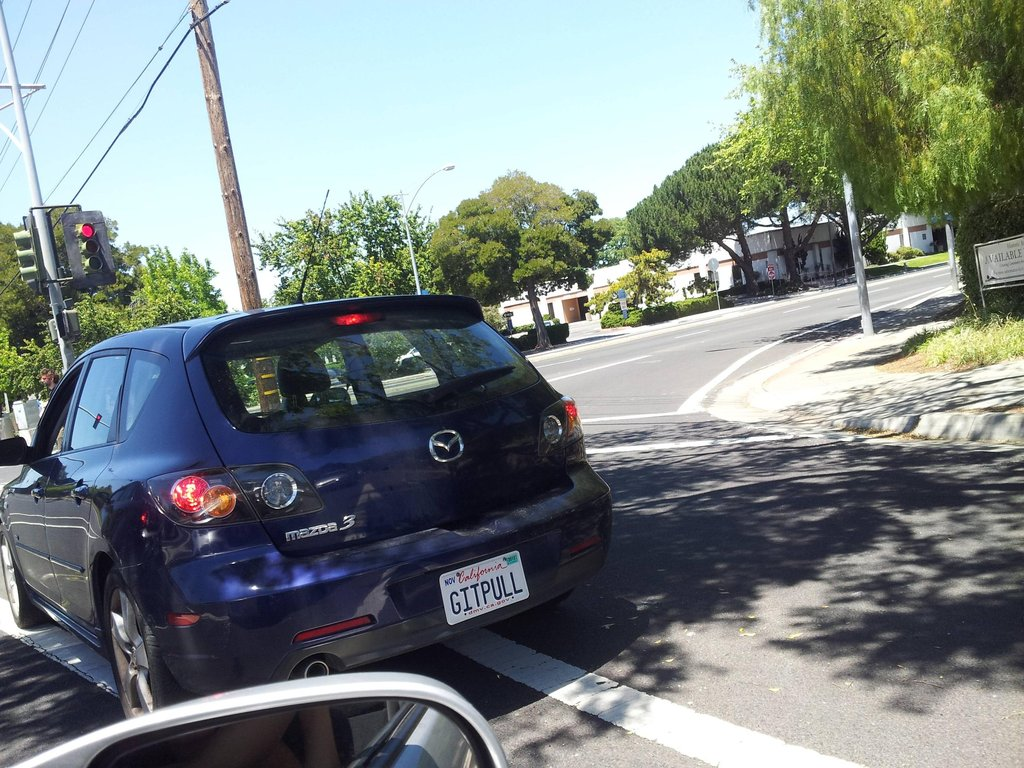
\includegraphics[width=\textwidth]{images/gitpull.jpg}
                \end{center}
            \end{figure}
        \end{column}
        \begin{column}{0.5\textwidth}
            \begin{lstlisting}
git pull origin master
            \end{lstlisting}
        \end{column}
    \end{columns} 
\end{frame}

\begin{frame}[fragile]
    \frametitle{Tutorial: Git}
    After years of using git, you might find this funny: 
    \begin{columns}
        \begin{column}{0.5\textwidth}
            \begin{figure}
                \begin{center}
                    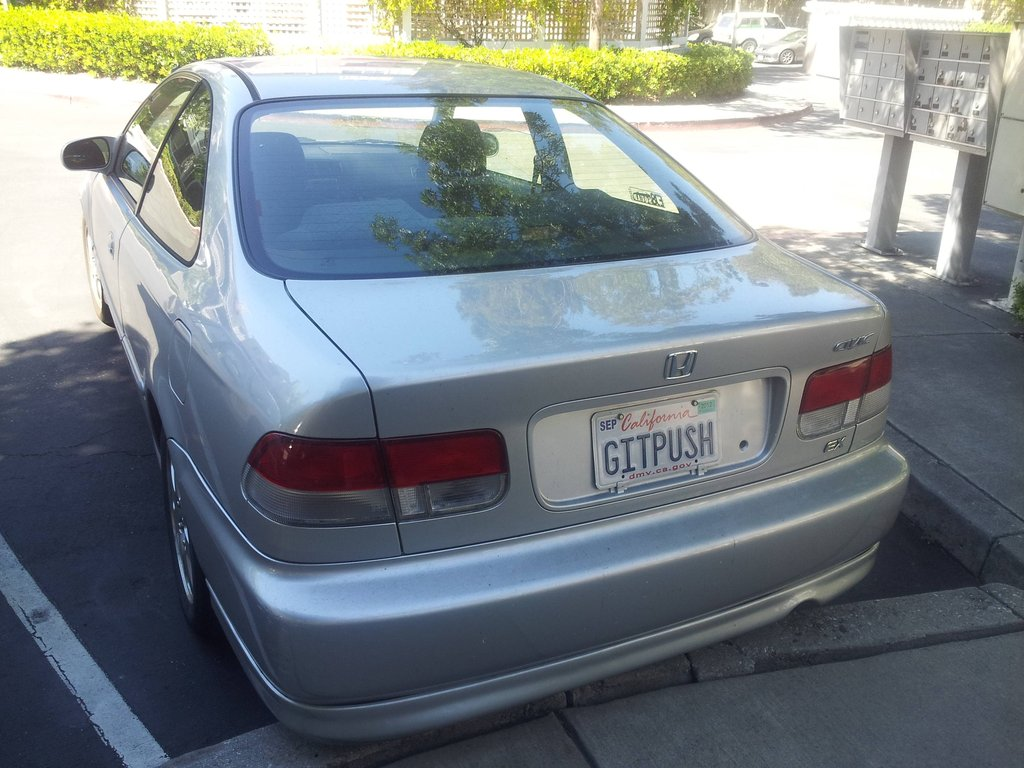
\includegraphics[width=\textwidth]{images/gitpush.jpg}
                \end{center}
            \end{figure}
        \end{column}
        \begin{column}{0.5\textwidth}
            \begin{lstlisting}
git push origin master
            \end{lstlisting}
        \end{column}
    \end{columns} 
\end{frame}

\begin{frame}[fragile]
    \frametitle{Tutorial: Git}
    \begin{columns}
        \begin{column}{0.4\textwidth}
            \begin{figure}
                \caption{For \$19.99, you can also have your own:}
                \begin{center}
                    
\includegraphics[width=\textwidth]{images/gitrdone.jpg}
                \end{center}
            \end{figure}
        \end{column}
        \begin{column}{0.6\textwidth}
\begin{lstlisting}
cd ~/
mkdir hub.git
mkdir computerA.git
mkdir computerB.git

git init --bare hub.git

cd hub.git
cd hooks
cp post-update.sample post-update
\end{lstlisting}
        \end{column}
    \end{columns} 
\end{frame}

\begin{frame}[fragile]
    \frametitle{Tutorial: Git}
    \begin{columns}
        \begin{column}{0.5\textwidth}
\begin{lstlisting}
cd computerA.git
git init 
git remote add origin ~/hub.git
echo 'Hello A' >> commonfile.txt
git add commonfile.txt 
git commit -am 'from A'
git pull origin master
git push origin master
\end{lstlisting}
        \end{column}
        \begin{column}{0.5\textwidth}
\begin{lstlisting}
cd computerB.git
git init 
git remote add origin ~/hub.git
echo ' World B' >> commonfile.txt
git add commonfile.txt 
git commit -am 'from B'
git pull origin master
git push origin master
\end{lstlisting}
        \end{column}
    \end{columns} 
\end{frame}


\begin{frame}[fragile]
    \frametitle{Tutorial: Git}
    \begin{columns}
        \begin{column}{0.5\textwidth}
    \begin{lstlisting}
cd ~/550400

git gui
git reset --hard HEAD

git branch personal
git branch
git checkout personal

edit some file 
git status 
git add . 
git commit -am 'personal edit'

git checkout master
git branch -D personal
    \end{lstlisting}
        \end{column}
        \begin{column}{0.5\textwidth}
    \begin{itemize}
        \item checks if there has been any change to the folder
        \item build and update the \texttt{master} git branch
        \item create and update a \texttt{personal} git branch
    \end{itemize}
        \end{column}
    \end{columns} 
\end{frame}



\begin{frame}
    \frametitle{Tutorial: Git}
    \texttt{.gitignore}?
    \vskip0.1in
    \begin{itemize}
        \item N.B.~the course folder already has one 
        \item Use it to let \emph{git} know the files to \emph{ignore} while
            version controlling
        \item one particular usage: create \texttt{.gitignore} at the root of
            your git folder 
        \item files already been list under the git watch list will not be
            ignored even after creation of \texttt{.gitignore} 
    \end{itemize}
\end{frame}

\subsection{Vim}

\newtheorem{DEFVim}{Vim}
\begin{frame}
    \frametitle{Vim}
    \begin{DEFVim}
        Vim is a \emph{highly customizable} text editor 
    \end{DEFVim}
    \vskip0.1in
    \begin{enumerate}
        \item \LaTeX, R, C/C++, Java, Python, Git and etc.
        \item Regular expression, syntax coloring, autocompletion
        \item Try Firefox + Wasavi/Vimperator/Vimium
        \item \texttt{<ESC>}-mode
        \begin{itemize}
            \item \texttt{:}-mode, aka., the last line mode
            \item \texttt{i}-mode, aka., the insert mode
        \end{itemize}
    \end{enumerate}
\end{frame}

\begin{frame}
    \frametitle{Tutorial: Vi}
    \begin{figure}
        \begin{center}
            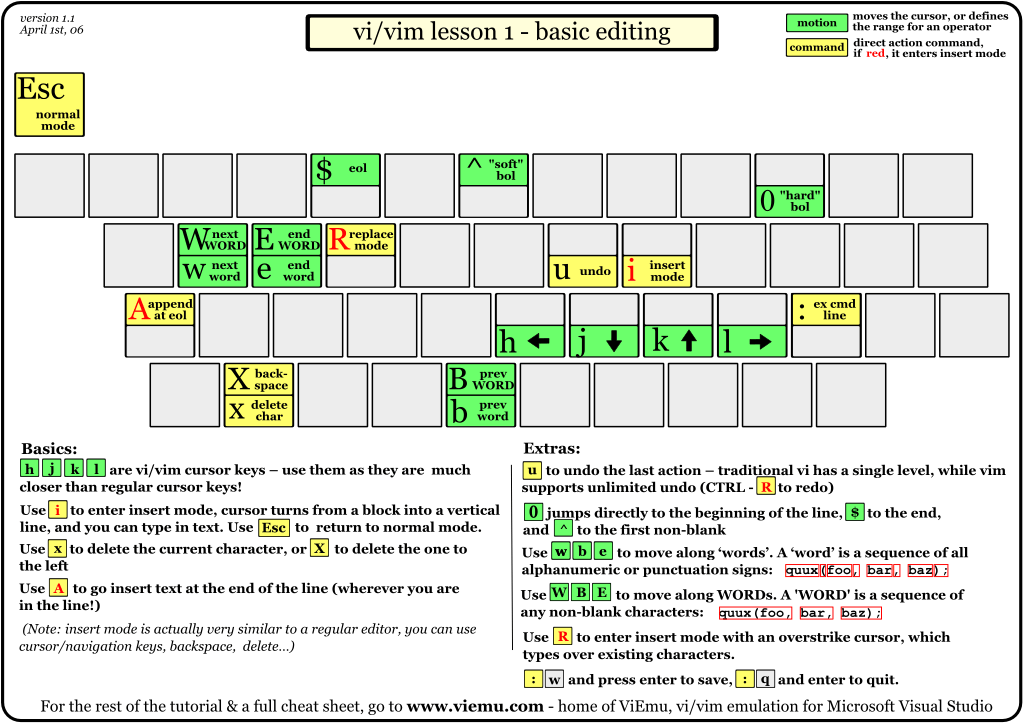
\includegraphics[width=\textwidth]{images/vi-vim-tutorial-1.png}
        \end{center}
        \caption{Vim Key}
        \label{fig:}
    \end{figure}
\end{frame}

\begin{frame}
    \frametitle{Tutorial: Vi}
    \begin{figure}
        \begin{center}
            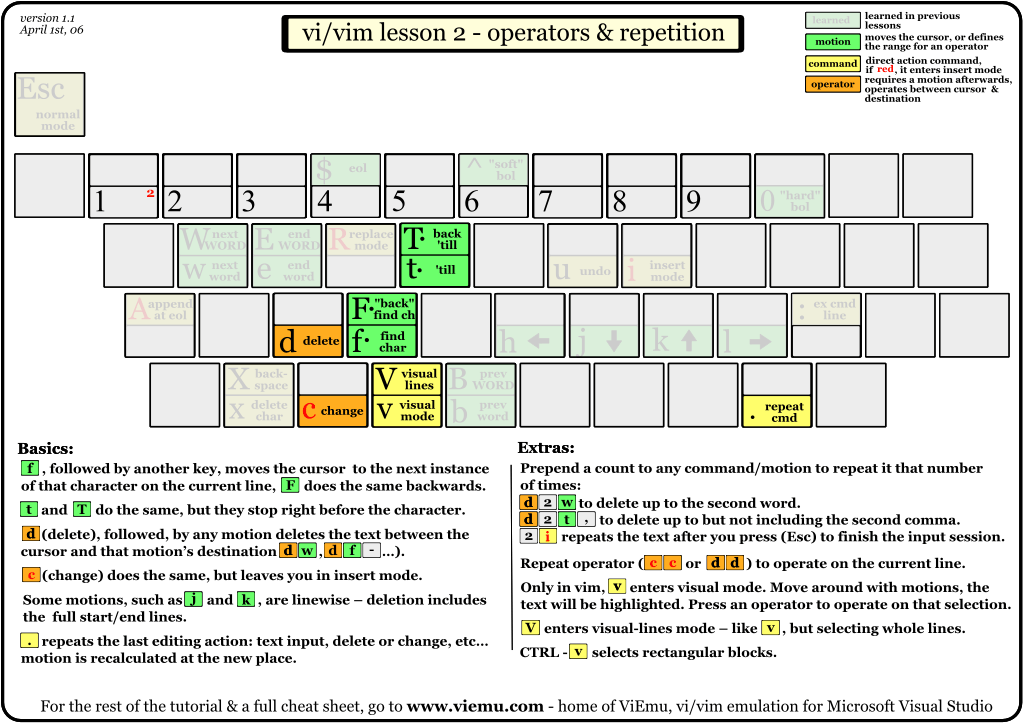
\includegraphics[width=\textwidth]{images/vi-vim-tutorial-2.png}
        \end{center}
        \caption{Vim Key}
        \label{fig:}
    \end{figure}
\end{frame}

\begin{frame}
    \frametitle{Tutorial: Vi}
    \begin{figure}
        \begin{center}
            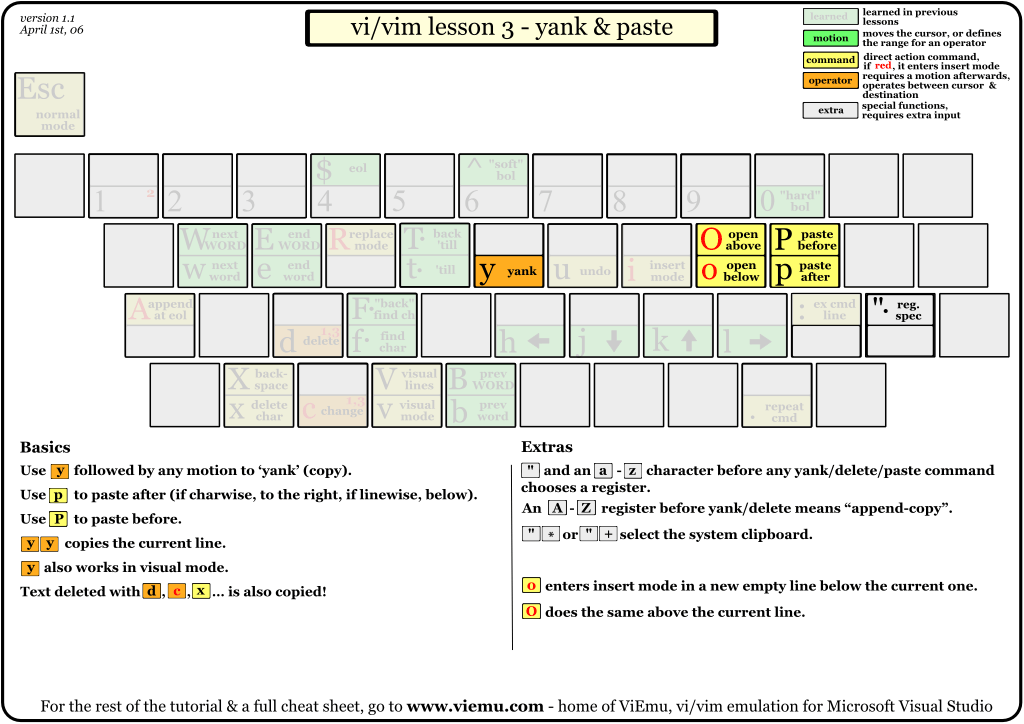
\includegraphics[width=\textwidth]{images/vi-vim-tutorial-3.png}
        \end{center}
        \caption{Vim Key}
        \label{fig:}
    \end{figure}
\end{frame}
\begin{frame}
    \frametitle{Tutorial: Vi}
    \begin{figure}
        \begin{center}
            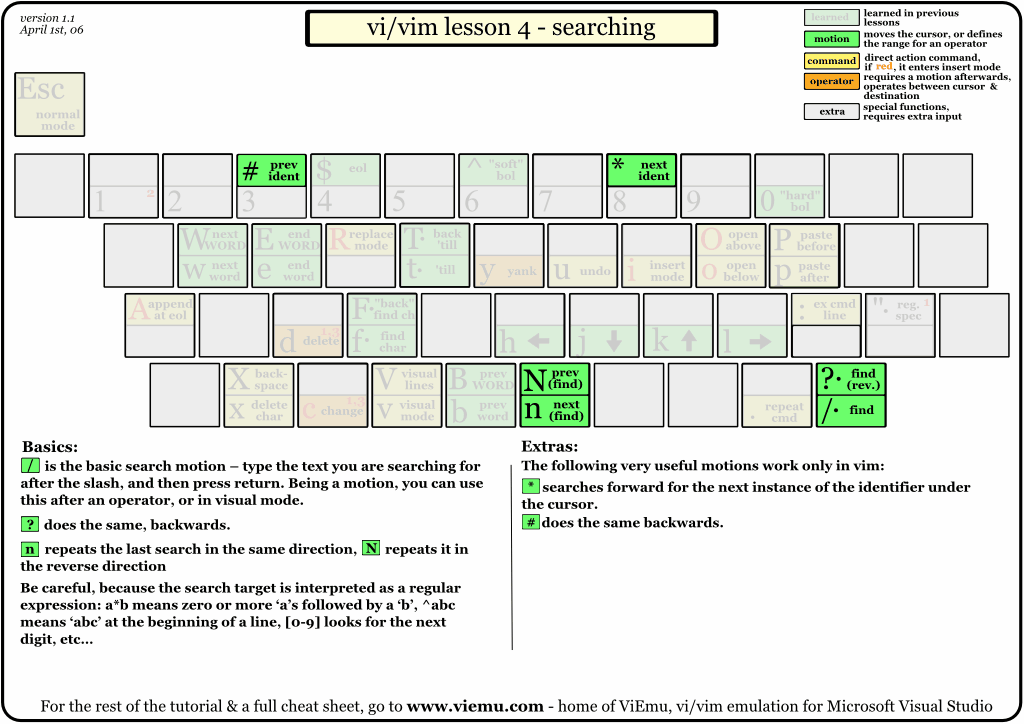
\includegraphics[width=\textwidth]{images/vi-vim-tutorial-4.png}
        \end{center}
        \caption{Vim Key}
        \label{fig:}
    \end{figure}
\end{frame}
\begin{frame}
    \frametitle{Tutorial: Vi}
    \begin{figure}
        \begin{center}
            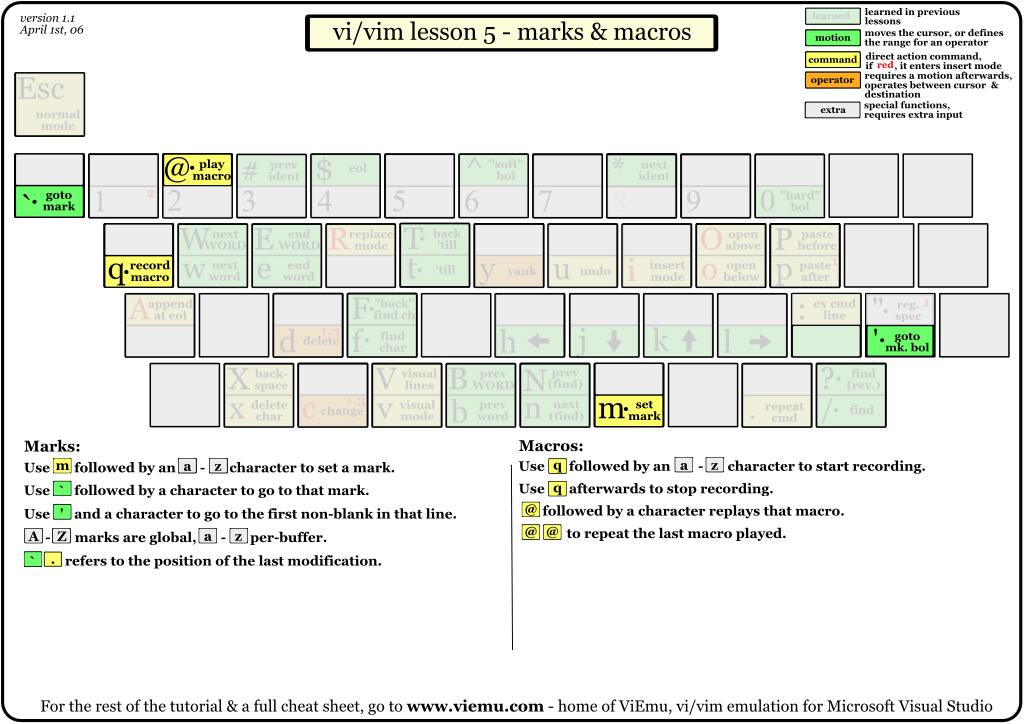
\includegraphics[width=\textwidth]{images/vi-vim-tutorial-5.png}
        \end{center}
        \caption{Vim Key}
        \label{fig:}
    \end{figure}
\end{frame}

\begin{frame}
    \frametitle{Tutorial: Vi}
    \begin{figure}
        \begin{center}
            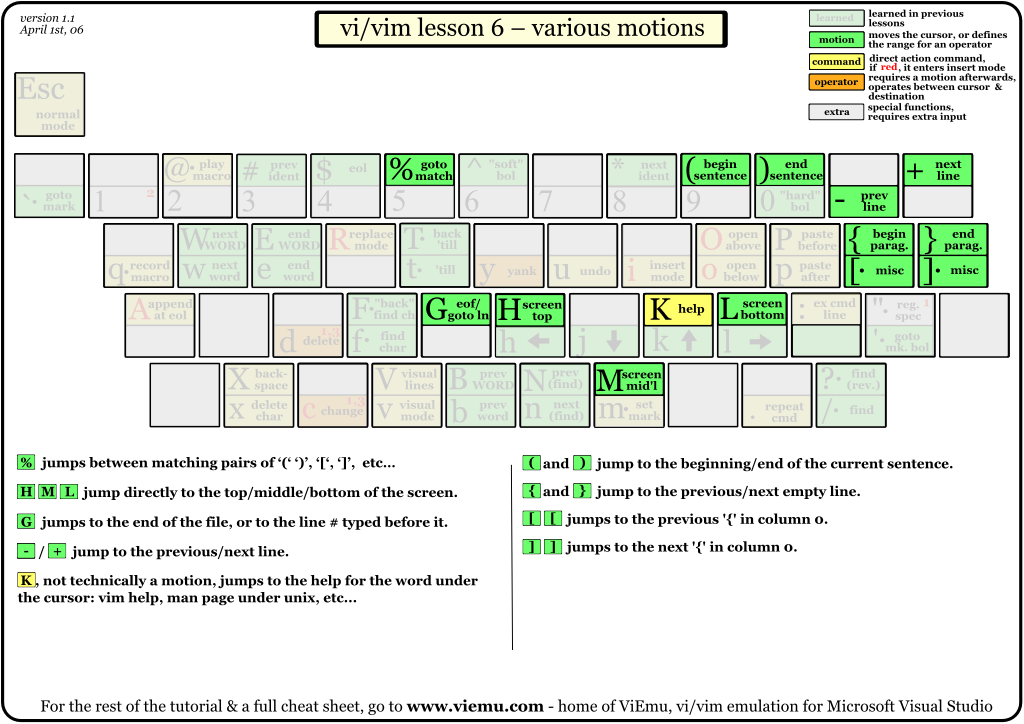
\includegraphics[width=\textwidth]{images/vi-vim-tutorial-6.png}
        \end{center}
        \caption{Vim Key}
        \label{fig:}
    \end{figure}
\end{frame}

\begin{frame}
    \frametitle{Tutorial: Vi}
    \begin{figure}
        \begin{center}
            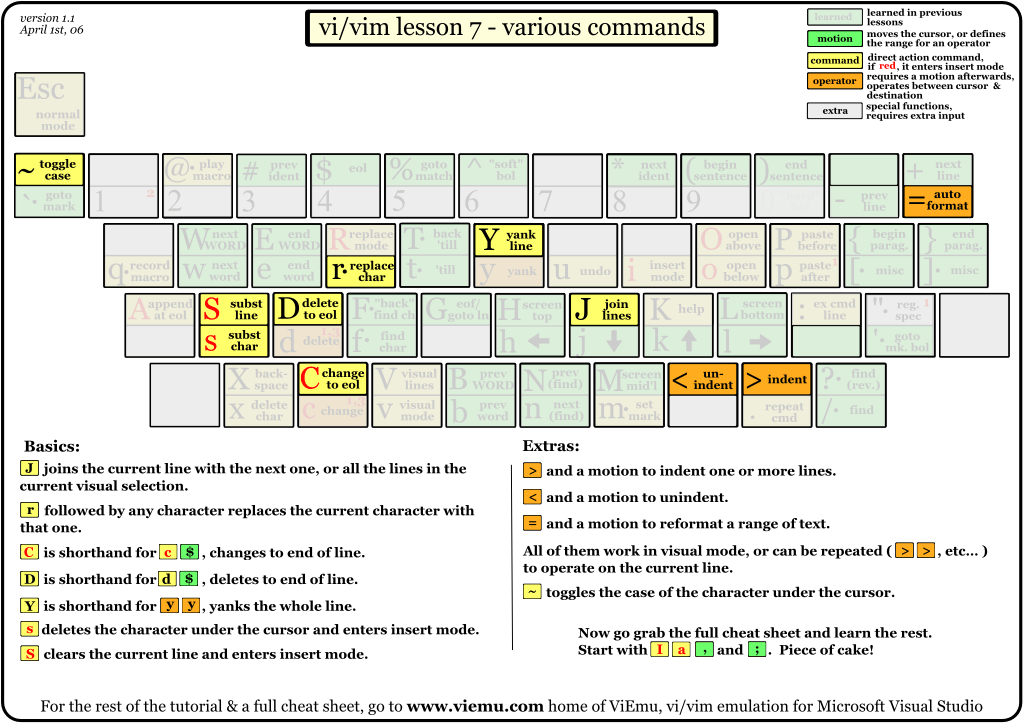
\includegraphics[width=\textwidth]{images/vi-vim-tutorial-7.png}
        \end{center}
        \caption{Vim Key}
        \label{fig:}
    \end{figure}
\end{frame}


\subsection{R}

\begin{frame}[fragile]
    \frametitle{Demo: R + \LaTeX}
    \begin{columns}
        \begin{column}{0.5\textwidth}
            \begin{figure}
                \centering
            \caption{R Studio}
            \href{http://rstudio.org}{
            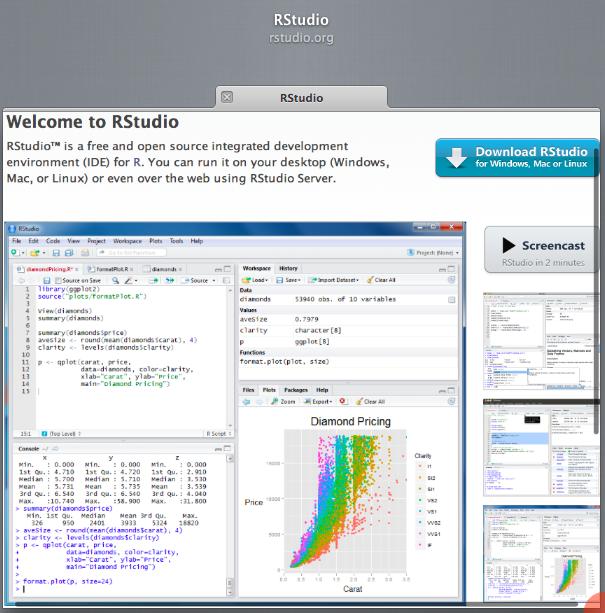
\includegraphics[width=\textwidth]{images/Rstudio}
            }
        \end{figure}
        \end{column}
        \begin{column}{0.5\textwidth}
            \begin{figure}
                \centering
                        \caption{R}
                    \href{http://www.r-project.org}{
                        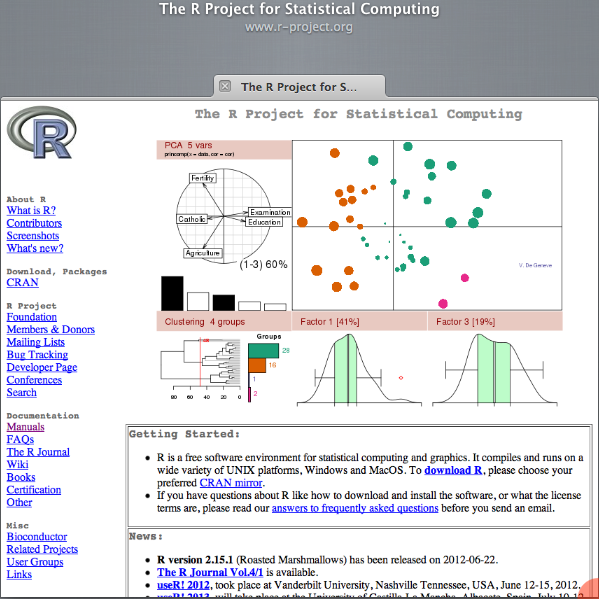
\includegraphics[width=\textwidth]{images/Rproject}}
            \end{figure}
        \end{column}
    \end{columns} 
\end{frame}

\begin{frame}[fragile]
    \frametitle{Demo: R + \LaTeX}
    \begin{columns}
        \begin{column}{0.45\textwidth}
    \begin{lstlisting}
install.packages(faraway)
install.packages(tikzDevice)
require(faraway)
require(tikzDevice)
data(eco)
tikz('embeddedfig1.tex', 
    standAlone=F, 
    width=5,height=5)
plot(income ~ usborn, 
    data=eco,
    xlab=`Proportion US born'
    ylab=`Mean Annual Income'
    )
dev.off()
    \end{lstlisting}
        \end{column}
        \begin{column}{0.55\textwidth}
        \begin{figure}[0.8\textwidth]
            % Created by tikzDevice version 0.6.2 on 2012-09-11 12:28:03
% !TEX encoding = UTF-8 Unicode
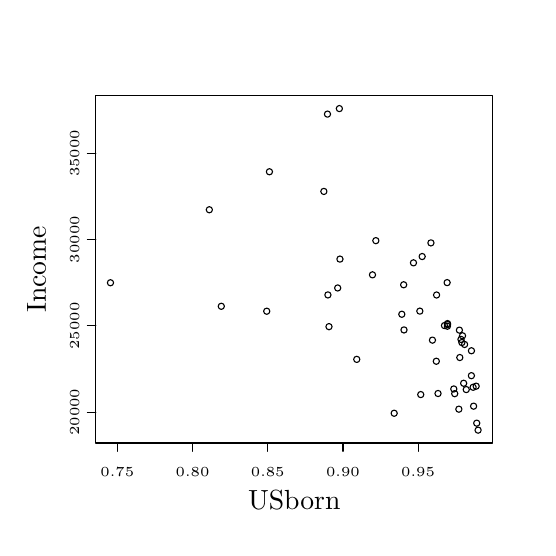
\begin{tikzpicture}[x=1pt,y=1pt,scale=0.5]
\definecolor[named]{drawColor}{rgb}{0.00,0.00,0.00}
\definecolor[named]{fillColor}{rgb}{1.00,1.00,1.00}
\fill[color=fillColor,fill opacity=0.00,] (0,0) rectangle (361.35,361.35);
\begin{scope}
\path[clip] ( 49.20, 61.20) rectangle (336.15,312.15);
\definecolor[named]{fillColor}{rgb}{0.00,0.00,0.00}
\definecolor[named]{drawColor}{rgb}{0.00,0.00,0.00}

\draw[color=drawColor,line cap=round,line join=round,fill opacity=0.00,] (321.92,101.46) circle (  2.25);

\draw[color=drawColor,line cap=round,line join=round,fill opacity=0.00,] (270.39,154.23) circle (  2.25);

\draw[color=drawColor,line cap=round,line join=round,fill opacity=0.00,] (237.82,121.63) circle (  2.25);

\draw[color=drawColor,line cap=round,line join=round,fill opacity=0.00,] (322.27, 87.80) circle (  2.25);

\draw[color=drawColor,line cap=round,line join=round,fill opacity=0.00,] ( 59.83,177.01) circle (  2.25);

\draw[color=drawColor,line cap=round,line join=round,fill opacity=0.00,] (278.80,191.40) circle (  2.25);

\draw[color=drawColor,line cap=round,line join=round,fill opacity=0.00,] (225.25,302.86) circle (  2.25);

\draw[color=drawColor,line cap=round,line join=round,fill opacity=0.00,] (291.43,205.82) circle (  2.25);

\draw[color=drawColor,line cap=round,line join=round,fill opacity=0.00,] (216.67,298.87) circle (  2.25);

\draw[color=drawColor,line cap=round,line join=round,fill opacity=0.00,] (172.76,156.43) circle (  2.25);

\draw[color=drawColor,line cap=round,line join=round,fill opacity=0.00,] (301.22,146.06) circle (  2.25);

\draw[color=drawColor,line cap=round,line join=round,fill opacity=0.00,] (139.93,159.99) circle (  2.25);

\draw[color=drawColor,line cap=round,line join=round,fill opacity=0.00,] (296.56, 96.96) circle (  2.25);

\draw[color=drawColor,line cap=round,line join=round,fill opacity=0.00,] (225.68,194.09) circle (  2.25);

\draw[color=drawColor,line cap=round,line join=round,fill opacity=0.00,] (313.14,136.08) circle (  2.25);

\draw[color=drawColor,line cap=round,line join=round,fill opacity=0.00,] (315.76,132.41) circle (  2.25);

\draw[color=drawColor,line cap=round,line join=round,fill opacity=0.00,] (303.32,145.58) circle (  2.25);

\draw[color=drawColor,line cap=round,line join=round,fill opacity=0.00,] (324.10,102.26) circle (  2.25);

\draw[color=drawColor,line cap=round,line join=round,fill opacity=0.00,] (307.96,100.26) circle (  2.25);

\draw[color=drawColor,line cap=round,line join=round,fill opacity=0.00,] (295.32,120.28) circle (  2.25);

\draw[color=drawColor,line cap=round,line join=round,fill opacity=0.00,] (251.62,207.43) circle (  2.25);

\draw[color=drawColor,line cap=round,line join=round,fill opacity=0.00,] (214.06,243.01) circle (  2.25);

\draw[color=drawColor,line cap=round,line join=round,fill opacity=0.00,] (283.42,156.50) circle (  2.25);

\draw[color=drawColor,line cap=round,line join=round,fill opacity=0.00,] (303.14,177.10) circle (  2.25);

\draw[color=drawColor,line cap=round,line join=round,fill opacity=0.00,] (325.52, 70.49) circle (  2.25);

\draw[color=drawColor,line cap=round,line join=round,fill opacity=0.00,] (314.27,138.67) circle (  2.25);

\draw[color=drawColor,line cap=round,line join=round,fill opacity=0.00,] (311.62, 85.63) circle (  2.25);

\draw[color=drawColor,line cap=round,line join=round,fill opacity=0.00,] (312.00,142.75) circle (  2.25);

\draw[color=drawColor,line cap=round,line join=round,fill opacity=0.00,] (224.04,173.24) circle (  2.25);

\draw[color=drawColor,line cap=round,line join=round,fill opacity=0.00,] (285.10,195.95) circle (  2.25);

\draw[color=drawColor,line cap=round,line join=round,fill opacity=0.00,] (174.71,257.22) circle (  2.25);

\draw[color=drawColor,line cap=round,line join=round,fill opacity=0.00,] (264.86, 82.69) circle (  2.25);

\draw[color=drawColor,line cap=round,line join=round,fill opacity=0.00,] (131.29,229.76) circle (  2.25);

\draw[color=drawColor,line cap=round,line join=round,fill opacity=0.00,] (313.79,133.80) circle (  2.25);

\draw[color=drawColor,line cap=round,line join=round,fill opacity=0.00,] (315.08,104.36) circle (  2.25);

\draw[color=drawColor,line cap=round,line join=round,fill opacity=0.00,] (303.42,147.48) circle (  2.25);

\draw[color=drawColor,line cap=round,line join=round,fill opacity=0.00,] (308.62, 96.85) circle (  2.25);

\draw[color=drawColor,line cap=round,line join=round,fill opacity=0.00,] (271.97,142.90) circle (  2.25);

\draw[color=drawColor,line cap=round,line join=round,fill opacity=0.00,] (295.52,168.15) circle (  2.25);

\draw[color=drawColor,line cap=round,line join=round,fill opacity=0.00,] (216.98,168.21) circle (  2.25);

\draw[color=drawColor,line cap=round,line join=round,fill opacity=0.00,] (316.94, 99.80) circle (  2.25);

\draw[color=drawColor,line cap=round,line join=round,fill opacity=0.00,] (320.67,109.84) circle (  2.25);

\draw[color=drawColor,line cap=round,line join=round,fill opacity=0.00,] (320.71,127.85) circle (  2.25);

\draw[color=drawColor,line cap=round,line join=round,fill opacity=0.00,] (217.76,145.28) circle (  2.25);

\draw[color=drawColor,line cap=round,line join=round,fill opacity=0.00,] (284.06, 96.19) circle (  2.25);

\draw[color=drawColor,line cap=round,line join=round,fill opacity=0.00,] (292.53,135.53) circle (  2.25);

\draw[color=drawColor,line cap=round,line join=round,fill opacity=0.00,] (271.72,175.54) circle (  2.25);

\draw[color=drawColor,line cap=round,line join=round,fill opacity=0.00,] (249.19,182.72) circle (  2.25);

\draw[color=drawColor,line cap=round,line join=round,fill opacity=0.00,] (324.52, 75.53) circle (  2.25);

\draw[color=drawColor,line cap=round,line join=round,fill opacity=0.00,] (303.47,146.80) circle (  2.25);

\draw[color=drawColor,line cap=round,line join=round,fill opacity=0.00,] (312.30,122.96) circle (  2.25);
\end{scope}
\begin{scope}
\path[clip] (  0.00,  0.00) rectangle (361.35,361.35);
\definecolor[named]{fillColor}{rgb}{0.00,0.00,0.00}
\definecolor[named]{drawColor}{rgb}{0.00,0.00,0.00}

\draw[color=drawColor,line cap=round,line join=round,fill opacity=0.00,] ( 64.82, 61.20) -- (282.19, 61.20);

\draw[color=drawColor,line cap=round,line join=round,fill opacity=0.00,] ( 64.82, 61.20) -- ( 64.82, 55.20);

\draw[color=drawColor,line cap=round,line join=round,fill opacity=0.00,] (119.16, 61.20) -- (119.16, 55.20);

\draw[color=drawColor,line cap=round,line join=round,fill opacity=0.00,] (173.50, 61.20) -- (173.50, 55.20);

\draw[color=drawColor,line cap=round,line join=round,fill opacity=0.00,] (227.85, 61.20) -- (227.85, 55.20);

\draw[color=drawColor,line cap=round,line join=round,fill opacity=0.00,] (282.19, 61.20) -- (282.19, 55.20);

\node[color=drawColor,anchor=base,inner sep=0pt, outer sep=0pt, scale=  1.00] at ( 64.82, 37.20) {\tiny 0.75};
\node[color=drawColor,anchor=base,inner sep=0pt, outer sep=0pt, scale=  1.00] at (119.16, 37.20) {\tiny 0.80};
\node[color=drawColor,anchor=base,inner sep=0pt, outer sep=0pt, scale=  1.00] at (173.50, 37.20) {\tiny 0.85};
\node[color=drawColor,anchor=base,inner sep=0pt, outer sep=0pt, scale=  1.00] at (227.85, 37.20) {\tiny 0.90};
\node[color=drawColor,anchor=base,inner sep=0pt, outer sep=0pt, scale=  1.00] at (282.19, 37.20) {\tiny 0.95};

\draw[color=drawColor,line cap=round,line join=round,fill opacity=0.00,] ( 49.20, 83.48) -- ( 49.20,270.47);

\draw[color=drawColor,line cap=round,line join=round,fill opacity=0.00,] ( 49.20, 83.48) -- ( 43.20, 83.48);

\draw[color=drawColor,line cap=round,line join=round,fill opacity=0.00,] ( 49.20,145.81) -- ( 43.20,145.81);

\draw[color=drawColor,line cap=round,line join=round,fill opacity=0.00,] ( 49.20,208.14) -- ( 43.20,208.14);

\draw[color=drawColor,line cap=round,line join=round,fill opacity=0.00,] ( 49.20,270.47) -- ( 43.20,270.47);

\node[rotate= 90.00,color=drawColor,anchor=base,inner sep=0pt, outer sep=0pt,
scale=  1.00] at ( 37.20, 83.48) {\tiny 20000};

\node[rotate= 90.00,color=drawColor,anchor=base,inner sep=0pt, outer sep=0pt,
scale=  1.00] at ( 37.20,145.81) {\tiny 25000};

\node[rotate= 90.00,color=drawColor,anchor=base,inner sep=0pt, outer sep=0pt,
scale=  1.00] at ( 37.20,208.14) {\tiny 30000};

\node[rotate= 90.00,color=drawColor,anchor=base,inner sep=0pt, outer sep=0pt,
scale=  1.00] at ( 37.20,270.47) {\tiny 35000};

\draw[color=drawColor,line cap=round,line join=round,fill opacity=0.00,] ( 49.20, 61.20) --
	(336.15, 61.20) --
	(336.15,312.15) --
	( 49.20,312.15) --
	( 49.20, 61.20);
\end{scope}
\begin{scope}
\path[clip] (  0.00,  0.00) rectangle (361.35,361.35);
\definecolor[named]{fillColor}{rgb}{0.00,0.00,0.00}
\definecolor[named]{drawColor}{rgb}{0.00,0.00,0.00}

\node[color=drawColor,anchor=base,inner sep=0pt, outer sep=0pt, scale=  1.00]
at (192.67, 13.20) {USborn};

\node[rotate= 90.00,color=drawColor,anchor=base,inner sep=0pt, outer sep=0pt,
scale=  1.00] at ( 13.20,186.67) {Income};
\end{scope}
\end{tikzpicture}

        \end{figure}
        \end{column}
    \end{columns} 
\end{frame}

\begin{frame}[fragile]
    \frametitle{Demo: R + \LaTeX}
    \begin{columns}
        \begin{column}{0.45\textwidth}
            \begin{lstlisting}
tikz('embeddedfig2.tex', 
    standAlone=F, 
    width=5,height=5)
plot(income ~ usborn, 
    data = eco,
    xlab=`Proportion US born',
    ylab=`Mean Annual Income',
    xlim=c(0,1),
    ylim=c(15000,70000),
    xaxs='i')
g<-lm(income~usborn,eco)
abline(coef(g))
dev.off()
            \end{lstlisting}
        \end{column}
        \begin{column}{0.55\textwidth}
            % Created by tikzDevice version 0.6.2 on 2012-09-11 13:10:12
% !TEX encoding = UTF-8 Unicode
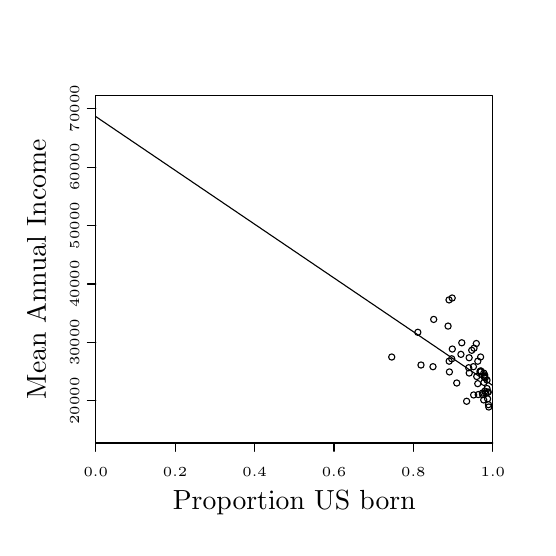
\begin{tikzpicture}[x=1pt,y=1pt,scale=0.5]
\definecolor[named]{drawColor}{rgb}{0.00,0.00,0.00}
\definecolor[named]{fillColor}{rgb}{1.00,1.00,1.00}
\fill[color=fillColor,fill opacity=0.00,] (0,0) rectangle (361.35,361.35);
\begin{scope}
\path[clip] ( 49.20, 61.20) rectangle (336.15,312.15);
\definecolor[named]{drawColor}{rgb}{0.00,0.00,0.00}

\draw[color=drawColor,line cap=round,line join=round,fill opacity=0.00,] (332.29, 97.71) circle (  2.25);

\draw[color=drawColor,line cap=round,line join=round,fill opacity=0.00,] (318.69,115.59) circle (  2.25);

\draw[color=drawColor,line cap=round,line join=round,fill opacity=0.00,] (310.09,104.55) circle (  2.25);

\draw[color=drawColor,line cap=round,line join=round,fill opacity=0.00,] (332.39, 93.08) circle (  2.25);

\draw[color=drawColor,line cap=round,line join=round,fill opacity=0.00,] (263.10,123.32) circle (  2.25);

\draw[color=drawColor,line cap=round,line join=round,fill opacity=0.00,] (320.91,128.19) circle (  2.25);

\draw[color=drawColor,line cap=round,line join=round,fill opacity=0.00,] (306.77,165.97) circle (  2.25);

\draw[color=drawColor,line cap=round,line join=round,fill opacity=0.00,] (324.24,133.08) circle (  2.25);

\draw[color=drawColor,line cap=round,line join=round,fill opacity=0.00,] (304.51,164.61) circle (  2.25);

\draw[color=drawColor,line cap=round,line join=round,fill opacity=0.00,] (292.91,116.34) circle (  2.25);

\draw[color=drawColor,line cap=round,line join=round,fill opacity=0.00,] (326.83,112.83) circle (  2.25);

\draw[color=drawColor,line cap=round,line join=round,fill opacity=0.00,] (284.24,117.55) circle (  2.25);

\draw[color=drawColor,line cap=round,line join=round,fill opacity=0.00,] (325.60, 96.19) circle (  2.25);

\draw[color=drawColor,line cap=round,line join=round,fill opacity=0.00,] (306.88,129.10) circle (  2.25);

\draw[color=drawColor,line cap=round,line join=round,fill opacity=0.00,] (329.97,109.44) circle (  2.25);

\draw[color=drawColor,line cap=round,line join=round,fill opacity=0.00,] (330.67,108.20) circle (  2.25);

\draw[color=drawColor,line cap=round,line join=round,fill opacity=0.00,] (327.38,112.66) circle (  2.25);

\draw[color=drawColor,line cap=round,line join=round,fill opacity=0.00,] (332.87, 97.98) circle (  2.25);

\draw[color=drawColor,line cap=round,line join=round,fill opacity=0.00,] (328.61, 97.30) circle (  2.25);

\draw[color=drawColor,line cap=round,line join=round,fill opacity=0.00,] (325.27,104.09) circle (  2.25);

\draw[color=drawColor,line cap=round,line join=round,fill opacity=0.00,] (313.73,133.62) circle (  2.25);

\draw[color=drawColor,line cap=round,line join=round,fill opacity=0.00,] (303.82,145.68) circle (  2.25);

\draw[color=drawColor,line cap=round,line join=round,fill opacity=0.00,] (322.13,116.36) circle (  2.25);

\draw[color=drawColor,line cap=round,line join=round,fill opacity=0.00,] (327.33,123.35) circle (  2.25);

\draw[color=drawColor,line cap=round,line join=round,fill opacity=0.00,] (333.24, 87.22) circle (  2.25);

\draw[color=drawColor,line cap=round,line join=round,fill opacity=0.00,] (330.27,110.32) circle (  2.25);

\draw[color=drawColor,line cap=round,line join=round,fill opacity=0.00,] (329.57, 92.34) circle (  2.25);

\draw[color=drawColor,line cap=round,line join=round,fill opacity=0.00,] (329.67,111.70) circle (  2.25);

\draw[color=drawColor,line cap=round,line join=round,fill opacity=0.00,] (306.45,122.04) circle (  2.25);

\draw[color=drawColor,line cap=round,line join=round,fill opacity=0.00,] (322.57,129.73) circle (  2.25);

\draw[color=drawColor,line cap=round,line join=round,fill opacity=0.00,] (293.43,150.50) circle (  2.25);

\draw[color=drawColor,line cap=round,line join=round,fill opacity=0.00,] (317.23, 91.35) circle (  2.25);

\draw[color=drawColor,line cap=round,line join=round,fill opacity=0.00,] (281.96,141.19) circle (  2.25);

\draw[color=drawColor,line cap=round,line join=round,fill opacity=0.00,] (330.15,108.67) circle (  2.25);

\draw[color=drawColor,line cap=round,line join=round,fill opacity=0.00,] (330.49, 98.69) circle (  2.25);

\draw[color=drawColor,line cap=round,line join=round,fill opacity=0.00,] (327.41,113.31) circle (  2.25);

\draw[color=drawColor,line cap=round,line join=round,fill opacity=0.00,] (328.78, 96.15) circle (  2.25);

\draw[color=drawColor,line cap=round,line join=round,fill opacity=0.00,] (319.11,111.75) circle (  2.25);

\draw[color=drawColor,line cap=round,line join=round,fill opacity=0.00,] (325.32,120.31) circle (  2.25);

\draw[color=drawColor,line cap=round,line join=round,fill opacity=0.00,] (304.59,120.33) circle (  2.25);

\draw[color=drawColor,line cap=round,line join=round,fill opacity=0.00,] (330.98, 97.15) circle (  2.25);

\draw[color=drawColor,line cap=round,line join=round,fill opacity=0.00,] (331.96,100.55) circle (  2.25);

\draw[color=drawColor,line cap=round,line join=round,fill opacity=0.00,] (331.97,106.65) circle (  2.25);

\draw[color=drawColor,line cap=round,line join=round,fill opacity=0.00,] (304.79,112.56) circle (  2.25);

\draw[color=drawColor,line cap=round,line join=round,fill opacity=0.00,] (322.30, 95.92) circle (  2.25);

\draw[color=drawColor,line cap=round,line join=round,fill opacity=0.00,] (324.53,109.26) circle (  2.25);

\draw[color=drawColor,line cap=round,line join=round,fill opacity=0.00,] (319.04,122.82) circle (  2.25);

\draw[color=drawColor,line cap=round,line join=round,fill opacity=0.00,] (313.09,125.25) circle (  2.25);

\draw[color=drawColor,line cap=round,line join=round,fill opacity=0.00,] (332.98, 88.92) circle (  2.25);

\draw[color=drawColor,line cap=round,line join=round,fill opacity=0.00,] (327.42,113.08) circle (  2.25);

\draw[color=drawColor,line cap=round,line join=round,fill opacity=0.00,] (329.75,105.00) circle (  2.25);
\end{scope}
\begin{scope}
\path[clip] (  0.00,  0.00) rectangle (361.35,361.35);
\definecolor[named]{drawColor}{rgb}{0.00,0.00,0.00}

\draw[color=drawColor,line cap=round,line join=round,fill opacity=0.00,] ( 49.20, 61.20) -- (336.15, 61.20);

\draw[color=drawColor,line cap=round,line join=round,fill opacity=0.00,] ( 49.20, 61.20) -- ( 49.20, 55.20);

\draw[color=drawColor,line cap=round,line join=round,fill opacity=0.00,] (106.59, 61.20) -- (106.59, 55.20);

\draw[color=drawColor,line cap=round,line join=round,fill opacity=0.00,] (163.98, 61.20) -- (163.98, 55.20);

\draw[color=drawColor,line cap=round,line join=round,fill opacity=0.00,] (221.37, 61.20) -- (221.37, 55.20);

\draw[color=drawColor,line cap=round,line join=round,fill opacity=0.00,] (278.76, 61.20) -- (278.76, 55.20);

\draw[color=drawColor,line cap=round,line join=round,fill opacity=0.00,] (336.15, 61.20) -- (336.15, 55.20);

\node[color=drawColor,anchor=base,inner sep=0pt, outer sep=0pt, scale=  1.00]
at ( 49.20, 37.20) {\tiny 0.0};

\node[color=drawColor,anchor=base,inner sep=0pt, outer sep=0pt, scale=  1.00] at (106.59, 37.20) {\tiny 0.2};

\node[color=drawColor,anchor=base,inner sep=0pt, outer sep=0pt, scale=  1.00] at (163.98, 37.20) {\tiny 0.4};

\node[color=drawColor,anchor=base,inner sep=0pt, outer sep=0pt, scale=  1.00] at (221.37, 37.20) {\tiny 0.6};

\node[color=drawColor,anchor=base,inner sep=0pt, outer sep=0pt, scale=  1.00] at (278.76, 37.20) {\tiny 0.8};

\node[color=drawColor,anchor=base,inner sep=0pt, outer sep=0pt, scale=  1.00] at (336.15, 37.20) {\tiny 1.0};

\draw[color=drawColor,line cap=round,line join=round,fill opacity=0.00,] ( 49.20, 91.62) -- ( 49.20,302.86);

\draw[color=drawColor,line cap=round,line join=round,fill opacity=0.00,] ( 49.20, 91.62) -- ( 43.20, 91.62);

\draw[color=drawColor,line cap=round,line join=round,fill opacity=0.00,] ( 49.20,133.87) -- ( 43.20,133.87);

\draw[color=drawColor,line cap=round,line join=round,fill opacity=0.00,] ( 49.20,176.11) -- ( 43.20,176.11);

\draw[color=drawColor,line cap=round,line join=round,fill opacity=0.00,] ( 49.20,218.36) -- ( 43.20,218.36);

\draw[color=drawColor,line cap=round,line join=round,fill opacity=0.00,] ( 49.20,260.61) -- ( 43.20,260.61);

\draw[color=drawColor,line cap=round,line join=round,fill opacity=0.00,] ( 49.20,302.86) -- ( 43.20,302.86);

\node[rotate= 90.00,color=drawColor,anchor=base,inner sep=0pt, outer sep=0pt,
scale=  1.00] at ( 37.20, 91.62) {\tiny 20000};

\node[rotate= 90.00,color=drawColor,anchor=base,inner sep=0pt, outer sep=0pt, scale=  1.00] at ( 37.20,133.87) {\tiny 30000};
\node[rotate= 90.00,color=drawColor,anchor=base,inner sep=0pt, outer sep=0pt, scale=  1.00] at ( 37.20,176.11) {\tiny 40000};
\node[rotate= 90.00,color=drawColor,anchor=base,inner sep=0pt, outer sep=0pt, scale=  1.00] at ( 37.20,218.36) {\tiny 50000};
\node[rotate= 90.00,color=drawColor,anchor=base,inner sep=0pt, outer sep=0pt, scale=  1.00] at ( 37.20,260.61) {\tiny 60000};
\node[rotate= 90.00,color=drawColor,anchor=base,inner sep=0pt, outer sep=0pt, scale=  1.00] at ( 37.20,302.86) {\tiny 70000};

\draw[color=drawColor,line cap=round,line join=round,fill opacity=0.00,] 
    ( 49.20, 61.20) --
	(336.15, 61.20) --
	(336.15,312.15) --
	( 49.20,312.15) --
	( 49.20, 61.20);
\end{scope}
\begin{scope}
\path[clip] (  0.00,  0.00) rectangle (361.35,361.35);
\definecolor[named]{drawColor}{rgb}{0.00,0.00,0.00}

\node[color=drawColor,anchor=base,inner sep=0pt, outer sep=0pt, scale=  1.00] at (192.68, 13.20) {Proportion US born};

\node[rotate= 90.00,color=drawColor,anchor=base,inner sep=0pt, outer sep=0pt, scale=  1.00] at ( 13.20,186.67) {Mean Annual Income};
\end{scope}
\begin{scope}
\path[clip] ( 49.20, 61.20) rectangle (336.15,312.15);
\definecolor[named]{drawColor}{rgb}{0.00,0.00,0.00}

\draw[color=drawColor,line cap=round,line join=round,fill opacity=0.00,] ( 49.20,297.12) -- (336.15,102.70);
\end{scope}
\end{tikzpicture}

        \end{column}
    \end{columns} 
\end{frame}
